\documentclass{article}
\usepackage[a4paper, margin=3mm, landscape]{geometry}
\usepackage{multicol}
\usepackage{xcolor}
\usepackage{enumitem}
\usepackage{amsmath}
\usepackage{amsfonts}
\usepackage{listings}
\usepackage{soul}
\usepackage{graphicx}

\pdfinfo{
    /Title (MA2104.pdf)
    /Creator (TeX)
    /Producer (pdfTeX 1.40.0)
    /Author (Jason Qiu)
    /Subject (MA2104)
    /Keywords (MA2104, nus, cheatsheet, pdf)
}

\graphicspath{ {./img/} }

\pagestyle{empty}
\setcounter{secnumdepth}{0}
\setlength{\columnseprule}{0.25pt}

% Redefine section commands to use less space
\makeatletter
\renewcommand{\section}{\@startsection{section}{1}{0mm}%
    {-1ex plus -.5ex minus -.2ex}%
    {0.5ex plus .2ex}%x
{\normalfont\large\bfseries}}
\renewcommand{\subsection}{\@startsection{subsection}{2}{0mm}%
    {-1explus -.5ex minus -.2ex}%
    {0.5ex plus .2ex}%
{\normalfont\normalsize\bfseries}}
\renewcommand{\subsubsection}{\@startsection{subsubsection}{3}{0mm}%
    {-1ex plus -.5ex minus -.2ex}%
    {1ex plus .2ex}%
{\normalfont\small\bfseries}}%
\makeatother

% Adjust spacing for all itemize/enumerate
\setlength{\leftmargini}{0.5cm}
\setlength{\leftmarginii}{0.5cm}
\setlist[itemize,1]{leftmargin=2mm,labelindent=1mm,labelsep=1mm}
\setlist[itemize,2]{leftmargin=2mm,labelindent=1mm,labelsep=1mm,label=$\bullet$}

% Font
\renewcommand{\familydefault}{\sfdefault}

% Define colors for math formulas
\definecolor{myblue}{cmyk}{1,.72,0,.38}
\everymath\expandafter{\the\everymath \color{myblue}}

% Custom command for keywords
\definecolor{highlight}{RGB}{251,243,218}
\newcommand{\keyword}[2][]{\sethlcolor{highlight}\hl{\textbf{#2}} #1 - }
\newcommand{\ilkeyword}[1]{\sethlcolor{highlight}\hl{\textbf{#1}}}

% Define colors and style for code
\definecolor{codegreen}{rgb}{0,0.6,0}
\definecolor{codegray}{rgb}{0.5,0.5,0.5}
\definecolor{codered}{HTML}{CC241D}
\definecolor{backcolor}{rgb}{0.95,0.95,0.95}
\lstdefinestyle{codestyle}{
    backgroundcolor = \color{backcolor},
    commentstyle = \color{codegray},
    keywordstyle = \color{codered},
    stringstyle = \color{codegreen},
    basicstyle = \ttfamily,
    breakatwhitespace = false,
    showstringspaces = false,
    breaklines = true,
    showtabs = false,
    tabsize = 2
}
\lstset{style = codestyle}

% -----------------------------------------------------------------------
\begin{document}
\begin{multicols*}{4}
\footnotesize

% Title box
\begin{center}
    \fbox{
        \parbox{0.8\linewidth}{
            \centering \textcolor{black}{
                {\Large\textbf{MA2104}} \\
                \normalsize{AY22/23 Sem 1}} \\
                {\footnotesize \textcolor{gray}{github.com/jasonqiu212}}
        }
    }
\end{center}

\section{01. Vectors, Lines, Planes}

\begin{itemize}
    \item \keyword{Dot Product}{$a \cdot b = ||a||||b|| \cos \theta$}
    \begin{itemize}
        \item $a \cdot b = b \cdot a$ $\quad$ $a \cdot (b + c) = a \cdot b + a \cdot c$ 
        \item $a \cdot b = 0 \leftrightarrow a \perp b$
    \end{itemize}
    \item \keyword{Projection}{$\text{proj}_{a}b = \frac{a \cdot b}{a \cdot a} a$}
    \begin{itemize}
        \item $\text{comp}_{a} b = ||\text{proj}_{a}b|| = \frac{a \cdot b}{||a||}$
    \end{itemize}
    \item \keyword{Cross Product}{$a \times b =
        \begin{vmatrix}
            i & j & k \\ 
            a_1 & a_2 & a_3 \\ 
            b_1 & b_2 & b_3 \\ 
        \end{vmatrix} = \langle a_2 b_3 - a_3 b_2, -(a_1 b_3 - b_1 a_3), a_1 b_2 - a_2 b_1 \rangle$}
    \begin{itemize}
        \item $a \times b \perp a$ and $\perp b$ $\quad$ $a \times b = - b \times a$
        \item $||a \times b|| = ||a||||b|| \sin \theta$ $\quad$ Direction: Right hand rule
        \item $A = ||a \times b||$ $\quad$ $||PQ||\sin \theta = \frac{||PQ \times PR||}{||PR||}$
    \end{itemize}
\end{itemize}

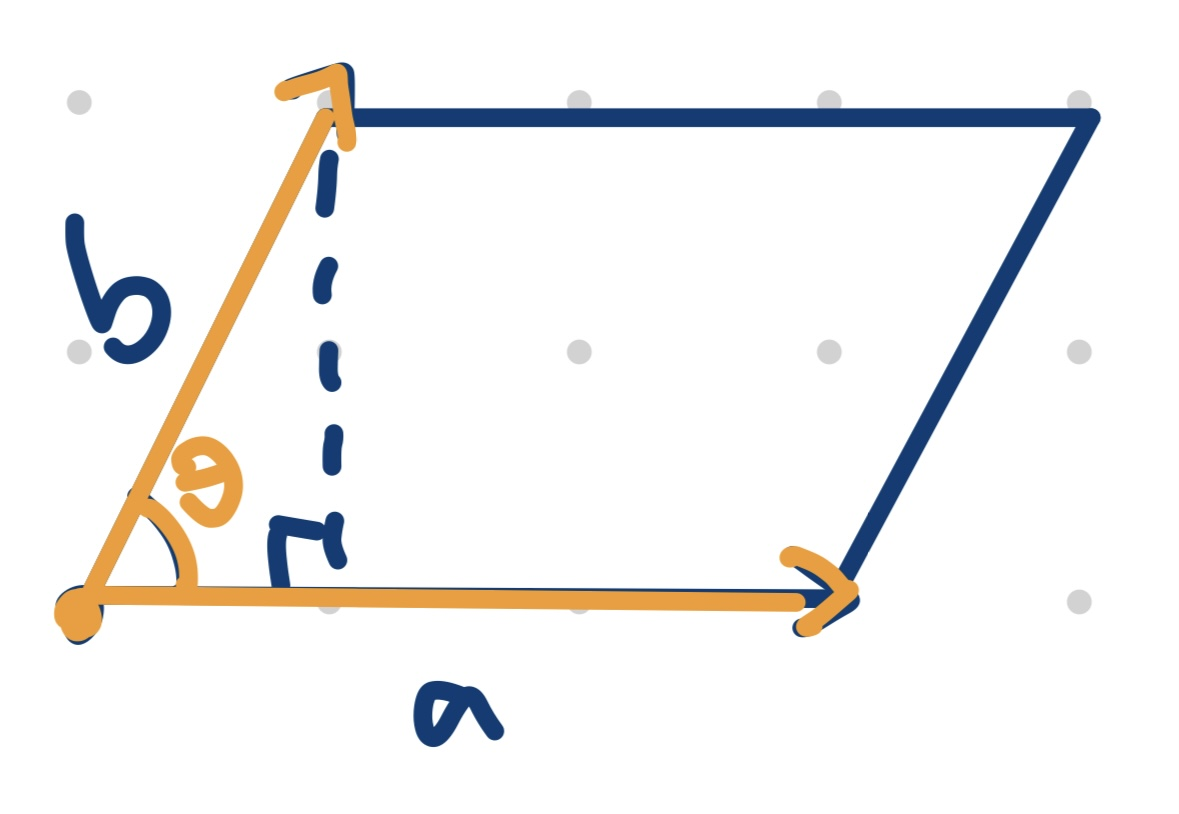
\includegraphics[scale=0.05]{area-of-parallelogram.jpg}
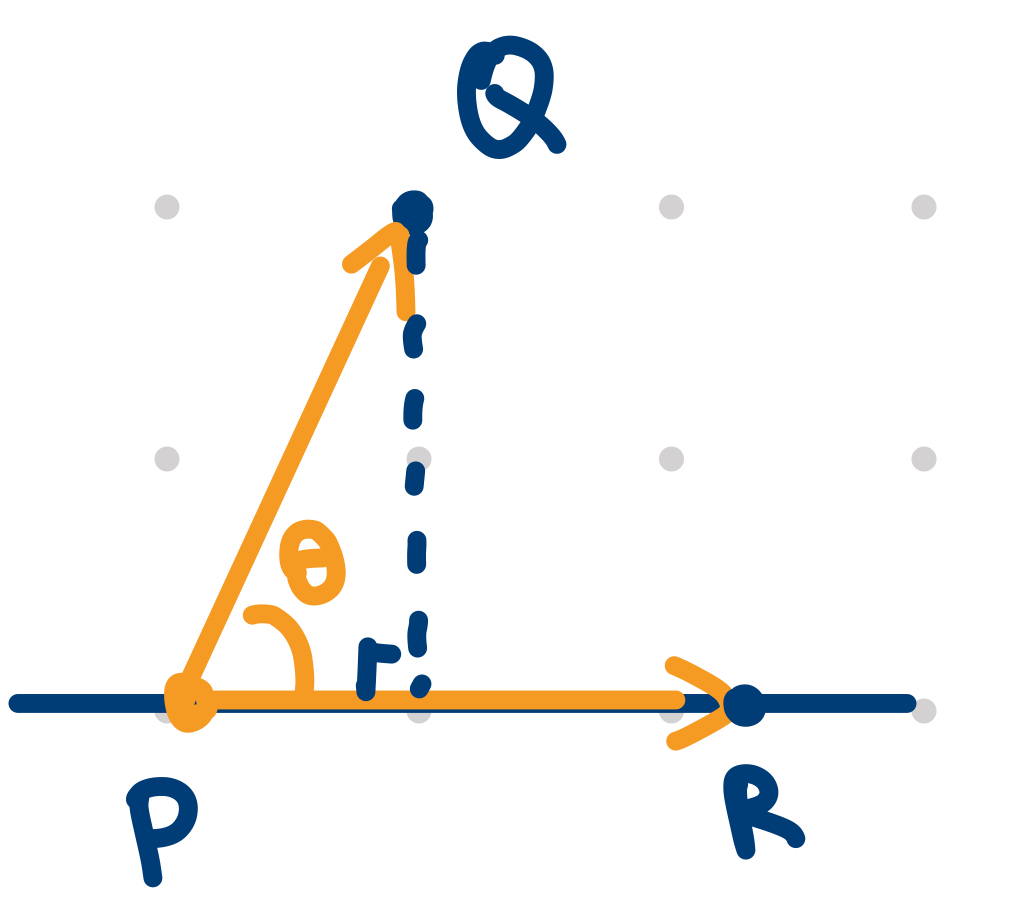
\includegraphics[scale=0.05]{distance-from-point-to-line.jpg}

\begin{itemize}
    \item \keyword{Scalar Triple Product}{$a \cdot (b \times c) = 
    \begin{vmatrix}
        a_1 & a_2 & a_3 \\ 
        b_1 & b_2 & b_3 \\ 
        c_1 & c_2 & c_3 \\ 
    \end{vmatrix}$}
    \begin{itemize}
        \item Result is a scalar value
        \item $A_{\text{Base}} = ||b \times c||$ $\quad$ $V = Ah = a \cdot (b \times c)$
    \end{itemize}
\end{itemize}

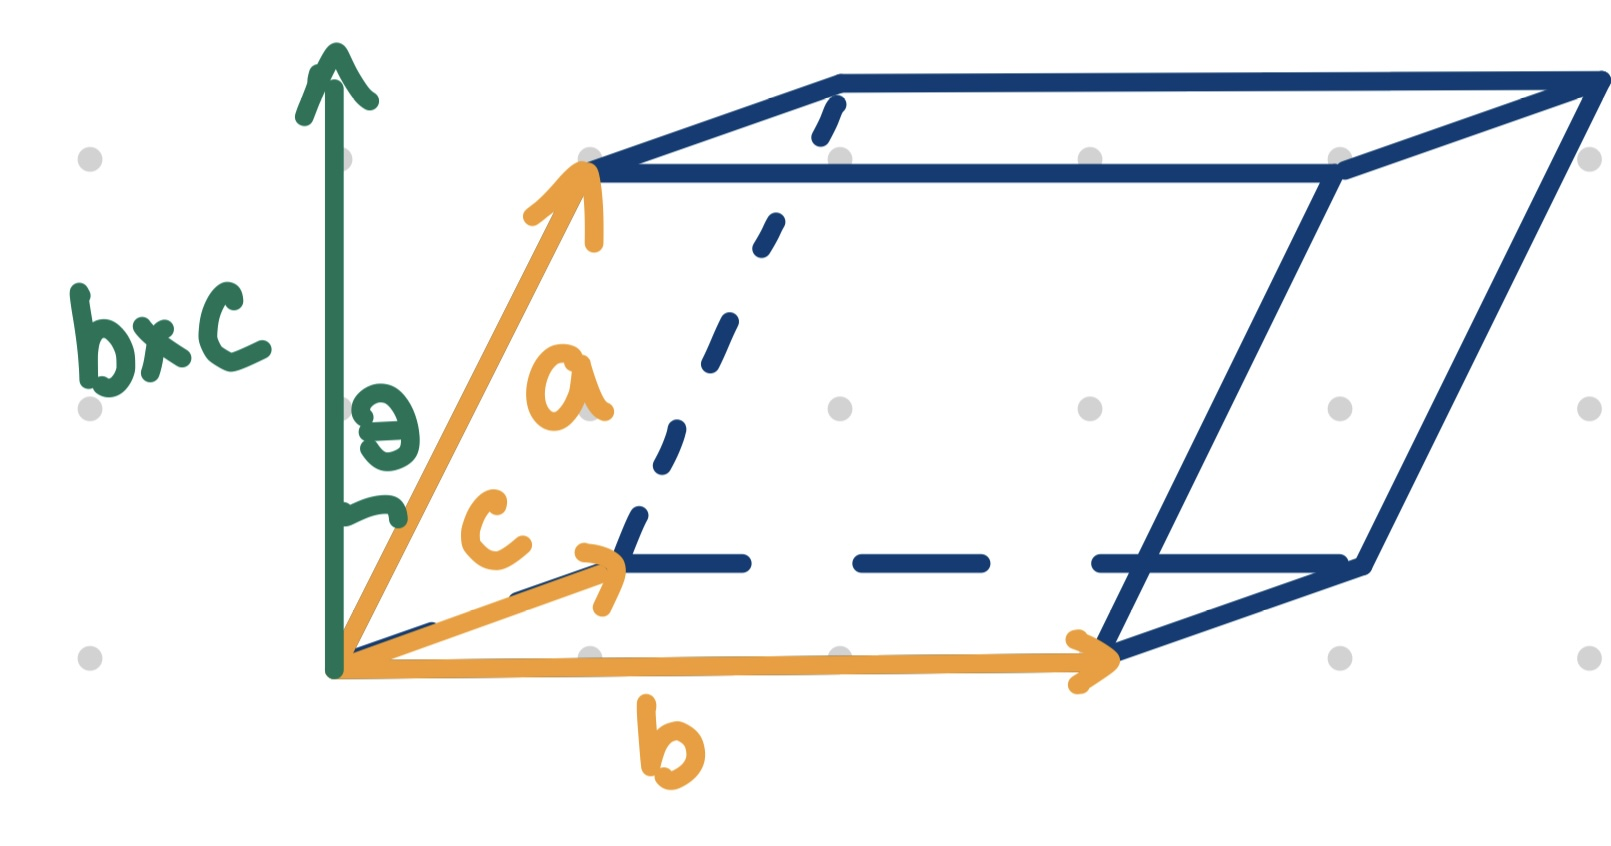
\includegraphics[scale=0.05]{volume-of-parallelepiped.jpg}

\begin{itemize}
    \item \keyword{Line}{$\langle x, y, z \rangle = \langle x_0, y_0, z_0 \rangle> + \langle a, b, c \rangle t$}
    \begin{itemize}
        \item 2D: Either parallel or intersecting
        \item 3D: Either parallel, intersecting, or skew
    \end{itemize}
    \item \keyword{Plane}{$\langle a,b,c \rangle \cdot \langle x,y,z \rangle = \langle a,b,c \rangle \cdot \langle x_0,y_0,z_0 \rangle$ where $\langle a,b,c \rangle$ is perpendicular to plane}
    \item \keyword{Tangent Vector}{Given $r(t) = \langle f(t),g(t),h(t) \rangle$:}
\end{itemize}

\[
    r'(a) = \lim_{\triangle{t} \rightarrow 0} \frac{r(a + \triangle{t}) - r(a)}{\triangle{t}} = \langle f'(a),g'(a),h'(a) \rangle
\]
\begin{itemize}
    \item $\frac{d}{dt}(r(t) + s(t)) = \frac{d}{dt} r(t) + \frac{d}{dt} s(t)$
    \item $\frac{d}{dt}(r(t)s(t)) = r'(t)s(t)+r(t)s'(t)$
    \item $\frac{d}{dt}(r(t) \cdot s(t)) = r'(t) \cdot s(t)+r(t) \cdot s'(t)$
    \item $\frac{d}{dt}(r(t) \times s(t)) = r'(t) \times s(t)+r(t) \times s'(t)$
    \item \keyword{Arc Length}{Given smooth $r(t) = \langle f(t),g(t),h(t) \rangle$:}
\end{itemize}

\[
    S = \int_{a}^{b} ||r'(t)|| dt
\]

\section{02. Functions of 2 Variables}

\section{03. Derivative}

\section{04. Gradient Vector}

\end{multicols*}
\end{document}
